\documentclass[12 pt]{article}
\usepackage{hyperref}
\usepackage[a4paper, left=2cm, right=2cm, top=2cm, bottom=2cm]{geometry}
\usepackage{graphicx}
\author{Pascal Hauser, Livio Näf}
\title{Bloom-Filter}
\begin{document}
\maketitle
\section{Idee des Bloom Filter: }
Man hat einen m-langen Bit-Array (gefüllt mit Nullen). Z.B. m=18
Ein Bloom-Filter hat ein Vokabular, dass ihm zugewiesen ist. (Menge von verschiedenen Werten)
Die \emph{k} unterschiedlichen Hashfunktionen stehen für die Anzahl Felder, welche im Bit-Array von 0 auf 1 gesetzt werden.
Für einen zu speichernden Wert z.B. \emph{"Hans"} werden \emph{k} Felder auf 1 gesetzt.
Um herauszufinden, ob nun ein Wert im Bit-Array bereits vorkommt, muss jeder der \emph{k} Stellen im Bit-Array auf 1 gesetzt sein. Falls einer der \emph{k} Stellen nicht 1 ist (also 0), so kann man sicher sagen, dass dieses Wort nicht in der Vorgegebenen Menge von Werten vorkommt.
Falls an jeder der \emph{k} Stellen eine 1 steht, ist es sehr wahrscheinlich dass dieser Wert bereits existiert. Man kann es aber nie mit 100 prozentiger Sicherheit sagen.
Es kann sein, dass der Bloom-Filter das Gefühl hat, dass ein Wert bereits vorhanden ist, wenn z.B. x1 setzt Stellen 0, 1, 3 auf den Wert 1. x2 setzt 1, 3, 7 auf den Wert 1. Und x3 setzt 0, 3, 7 welche bereits alle schon auf 1 gesetzt wurden (somit glaubt der Bloom-Filter, dass dieser Wert bereits vorkam, obwohl dies nicht der Fall ist.) = falsch positives Ergebnis. Durch das Anpassen der Paramter kann dieses Risiko minimiert werden!
\subsection{Vorteil:}
Man kann 100 Prozent sicher sein, dass ein Wert nicht vorkommt, wenn dies der Bloom-Filter sagt!
\subsection{Nachteile:}
\begin{itemize}
    \item{Es besteht immer ein minimales (trotz Anpassen der Parameter) Risiko, dass der Bloom-Filter fälschlicherweise sagt, dass ein Wert vorkommt.}
    \item{Bereits gesetzte Stellen im Bit-Array bleiben 1, egal was passiert}
\end{itemize}
\subsection{Konkretes Beispiel aus der Praxis: }
\begin{itemize}
    \item{Bloomfilter können von Nutzen sein, wenn sensible Daten gespeichert werden sollen. Beispielsweise kann das Verfahren dazu verwendet werden, um bei einer Fahndung sicher auszuschliessen, dass eine gerade überprüfte Person gesucht wird, ohne dabei Personendaten im Klartext vorhalten zu müssen.}
    \item{Google Chrome prüft anhand eines Bloomfilters mit den Signaturen gefährlicher Webseiten bereits bei der Eingabe der URL, ob diese im Filter enthalten und somit gefährlich ist.}
\end{itemize}
\pagebreak
\section{Implementation in Java}
\subsection{Überprüfen der Fehlerwahrscheinlichkeit p der Datenstruktur}
Um die Fehlerwahrscheinlichkeit der Datenstruktur zu überprüfen, wurden 1000000 Wörter mit der Funktion \emph{RandomStringUtils.random} welche im Package \emph{org.apache.commons.lang3} enthalten ist, generiert. Danach wurde die Wörter mit den gleichenHashfunktionen wie bei den Orignialwörtern gehasht. Wird ein Wort anhand der Hashwerte als "enthalten" identifiziert, wird im HashSet nachgeschaut, ob dieses tatsächlich im Set enthalten ist. Ist dies nicht der Fall, wird der Counter \emph{FalsePositive} inkrementiert.
\subsection{Konkrete Ausgabe}
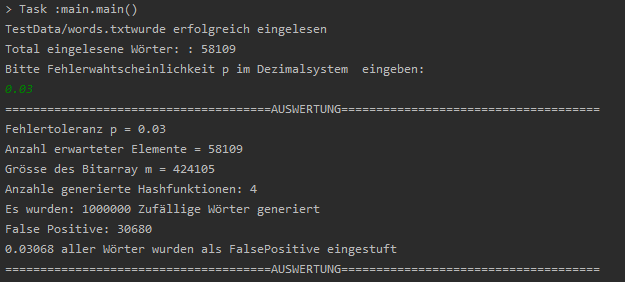
\includegraphics[width=0.7\textwidth]{Ausgabe_Java.png}
\subsubsection{Quellen}
https://www.youtube.com/watch?v=bEmBh1HtYrw
\linebreak https://de.wikipedia.org/wiki/Bloomfilter
\end{document}